% Fig. 4.3 -- 五條不同參數的貝塔分配密度曲線疊在同一張圖上。
% 書稿來源: mathstatch4.tex 第 3049 至 3077 行的 tikzpicture (置於 center 之內，內容
%   全部由 pgfplots 的 axis 環境畫出，width = .8\textwidth、height = .55\textwidth)。
%   書稿以 declare function 定義 (a+b-1)!/((a-1)!(b-1)!) * k^(a-1) * (1-k)^(b-1)，
%   即五組參數皆為正整數時的貝塔密度，samples = 600、domain 0:1、smooth;
%   只畫 x 軸 (axis x line=bottom)，y 軸不畫 (axis y line=none) 也不顯示刻度數值，
%   兩軸皆不寫軸名，xtick = {0, 0.1, ..., 1.1}，xmin = -0.1、xmax = 1.1、
%   ymin = 0、ymax = 4。五組參數依書稿的繪製順序與線型為
%     (1,1) thick 實線、(2,4) dashdotted、(2,2) 一般實線、(4,2) dashdotdotted、
%     (8,8) dashed，一律黑色，各以 \addlegendentry 標出參數。
%
% 各條曲線的係數 Gamma(a+b)/(Gamma(a)Gamma(b)) 與峰值:
%   (1,1)  f(x) = 1                    在 [0,1] 上為定值
%   (2,4)  f(x) = 20 x (1-x)^3         眾數 0.25，峰值 2.109375
%   (2,2)  f(x) = 6 x (1-x)            眾數 0.5， 峰值 1.5
%   (4,2)  f(x) = 20 x^3 (1-x)         眾數 0.75，峰值 2.109375
%   (8,8)  f(x) = 51480 x^7 (1-x)^7    眾數 0.5， 峰值 3.142090
% (8,8) 那一條改寫為 (4.7108573 x (1-x))^7 再逐項相乘，4.7108573 = 51480^(1/7)。
% 這是為了讓 pgfmath 的定點運算不必經過 6.1e-5 這一級距的中間值: 直接寫
% 51480*x^7*(1-x)^7 時，x^7 在 x = 0.5 附近會被截到 0.00006，峰值誤差達 1.7%。
%
% 對書稿的四處調整:
%
%   1. 五條曲線一律 journalink 0.8pt，改以線型分辨，不以粗細分辨。書稿的 (1,1) 與
%      (2,2) 都是實線、只差 thick 與否，在網頁的 0.8pt 統一線寬之下無法分辨，故
%      (2,2) 改為點線; 其餘三條保留書稿的 dashdotted、dashdotdotted、dashed 對應。
%      依 CH2_FIGURE_SPECS.md 1.9，多曲線比較不得只靠顏色分辨。
%   2. 圖例移到左上角，位置與版位逐條核算過。書稿以 pgfplots 的 \addlegendentry 出
%      圖例框; CH2_FIGURE_SPECS.md 1.9 以曲線末端直接標註為優先，但五條曲線在 x = 0
%      與 x = 1 兩端全部收斂到同一處，末端無法各自標註，故取該條所允許的圖例作法，
%      短線段樣本 0.5cm。圖例佔 x 自 -0.10 至約 0.32、y 自 2.30 至 4.09 這一塊:
%      (2,4) 的峰值 2.109375 是該塊之下最高的一條，(8,8) 要到 x = 0.392 才升到
%      2.25，都在圖例右緣之外，故五列都不壓到曲線。
%   3. 刻度數值只標 0、0.2、0.4、0.6、0.8、1，刻度線仍每 0.1 一格。書稿每 0.1 標一
%      個數值，在網頁的原生寬之下相鄰標籤只差 0.6cm，會相碰。書稿 xtick 到 1.1，
%      該處已在密度的定義域之外，只是軸線的延伸，故刻度線畫到 1.0 為止。
%   4. x 軸末端補上軸名 $x$ (書稿 xlabel 為空)，記號取候選稿內文的 f_X(x) 之 x。
%
% 取樣數由書稿的 600 降為 200，即 CH2_FIGURE_SPECS.md 1.6 所定的下限。三個取樣數各
% 產一次 SVG 的實測: 600 為 174,086 位元組 (gzip 72,521)、300 為 99,106 (gzip 32,451)、
% 200 為 74,240 (gzip 23,175)。600 已越過 CH4_FIGURE_SPECS.md 3.1 所定的 100 KB 分界。
% 200 與 600 在 300 dpi (964 x 709 px，約為 350 px 顯示寬的四倍) 之下逐點相減，
% 灰階差超過 8 的只有 214 點、最大差 27，全落在曲線邊緣，即消鋸齒的差異。
%
% 版面: x = 6cm、y = 1.3cm，原生寬約 8.0cm，在 CH2_FIGURE_SPECS.md 1.3 的 9.0cm
%   上限之內。圖內沒有 \scriptscriptstyle，最小字即 10pt 本文級。
%
% 產製:
%   pdflatex beta-density-family.tex
%   pdftocairo -svg beta-density-family.pdf ../../images/teaching-topics/beta-density-family.svg

\documentclass[tikz,border=2pt]{standalone}
\usepackage{amsmath}
\usepackage{amssymb}
\usepackage{xcolor}
\usetikzlibrary{arrows.meta}

\definecolor{journalink}{HTML}{1F1C18}
\definecolor{journalmuted}{HTML}{8A7F72}
\definecolor{journalaccent}{HTML}{9C2D2D}

\begin{document}
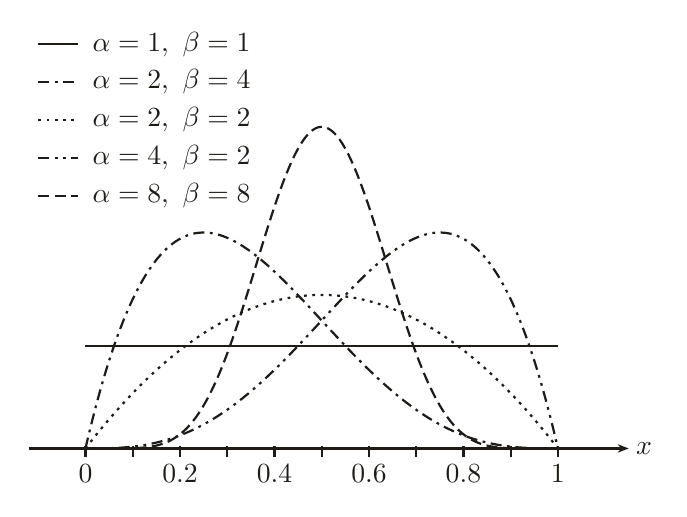
\begin{tikzpicture}[
  x=6cm, y=1.3cm,
  declare function={
    q88(\t) = 4.7108573*\t*(1-\t);
    b24(\t) = 20*\t*(1-\t)*(1-\t)*(1-\t);
    b22(\t) = 6*\t*(1-\t);
    b42(\t) = 20*\t*\t*\t*(1-\t);
    b88(\t) = q88(\t)*q88(\t)*q88(\t)*q88(\t)*q88(\t)*q88(\t)*q88(\t);
  },
  every node/.style={font=\normalsize, journalink},
  axis/.style={journalink, line width=0.8pt, -{Stealth[length=4pt]}},
  tick/.style={journalink, line width=0.8pt},
  cu/.style={journalink, line width=0.8pt},
  sOne/.style={cu},
  sTwoFour/.style={cu, dash pattern=on 4pt off 2pt on 1pt off 2pt},
  sTwoTwo/.style={cu, dash pattern=on 1pt off 2pt},
  sFourTwo/.style={cu, dash pattern=on 4pt off 2pt on 1pt off 2pt on 1pt off 2pt},
  sEight/.style={cu, dash pattern=on 4pt off 2pt}
]

  %% ---- 五條密度曲線 ------------------------------------------------
  \draw[sOne] (0,1) -- (1,1);
  \draw[sTwoFour] plot[domain=0:1, samples=200, smooth] (\x,{b24(\x)});
  \draw[sTwoTwo]  plot[domain=0:1, samples=200, smooth] (\x,{b22(\x)});
  \draw[sFourTwo] plot[domain=0:1, samples=200, smooth] (\x,{b42(\x)});
  \draw[sEight]   plot[domain=0:1, samples=200, smooth] (\x,{b88(\x)});

  %% ---- x 軸 ---------------------------------------------------------
  \draw[axis] (-0.12,0) -- (1.15,0);
  \node[anchor=west, inner sep=2.5pt] at (1.15,0) {$x$};

  \foreach \t in {0,0.1,0.2,0.3,0.4,0.5,0.6,0.7,0.8,0.9,1}
    \draw[tick] ([yshift=1pt]\t,0) -- ([yshift=-3pt]\t,0);
  \node[anchor=north, inner sep=2.5pt] at ([yshift=-3pt]0,0)   {$0$};
  \node[anchor=north, inner sep=2.5pt] at ([yshift=-3pt]0.2,0) {$0.2$};
  \node[anchor=north, inner sep=2.5pt] at ([yshift=-3pt]0.4,0) {$0.4$};
  \node[anchor=north, inner sep=2.5pt] at ([yshift=-3pt]0.6,0) {$0.6$};
  \node[anchor=north, inner sep=2.5pt] at ([yshift=-3pt]0.8,0) {$0.8$};
  \node[anchor=north, inner sep=2.5pt] at ([yshift=-3pt]1,0)   {$1$};

  %% ---- 圖例，左上角 -------------------------------------------------
  %% 短線段樣本 0.5cm，自 x = -0.10 到 x = -0.0166667。
  \draw[sOne]     (-0.1,3.95) -- (-0.0166667,3.95);
  \node[anchor=west, inner sep=1.5pt] at (0.005,3.95) {$\alpha=1,\ \beta=1$};

  \draw[sTwoFour] (-0.1,3.58) -- (-0.0166667,3.58);
  \node[anchor=west, inner sep=1.5pt] at (0.005,3.58) {$\alpha=2,\ \beta=4$};

  \draw[sTwoTwo]  (-0.1,3.21) -- (-0.0166667,3.21);
  \node[anchor=west, inner sep=1.5pt] at (0.005,3.21) {$\alpha=2,\ \beta=2$};

  \draw[sFourTwo] (-0.1,2.84) -- (-0.0166667,2.84);
  \node[anchor=west, inner sep=1.5pt] at (0.005,2.84) {$\alpha=4,\ \beta=2$};

  \draw[sEight]   (-0.1,2.47) -- (-0.0166667,2.47);
  \node[anchor=west, inner sep=1.5pt] at (0.005,2.47) {$\alpha=8,\ \beta=8$};

\end{tikzpicture}
\end{document}
